% Source: source_md/intelligence_part2_combined_ja.md
\section{非閉包定理 — 推論層 $L_F$ に内部不動点が存在しないこと}

\noindent\textbf{記述の射程。} 定理の議論は、明記された正当化の厳密増加と、固定拘束・領域内移動の範囲に条件づけられる。ここで証明妥当性の認証や普遍的認知解釈を与えるものではない。仮想的な二値停止述語は停止を不動点条件としてモデル化するが、任意の認知的終了への適用や、補助推論への前提再適用は未解決である。境界発散と不動点不在は役割の比較であり、証明された同型ではない。個体閉包不能、外部停止の必要性、崩壊regimeはそれぞれ別の構成・認知仮説である。



本章は本論文の第一中心である(第二中心は \S{}5)。保存する旧局所状態模型の範囲で、推論層 $L_F$ に\textbf{内部不動点が存在しないこと}を構造的命題として導出し、その動力学的帰結を述べる。

この形式的議論と、推論層 $L_F$ の認知的閉包不能という解釈は別である。停止の外部化は構成案であり、普遍的な必要性を導いたものではない。\S{}5 では、ログ層 $L_R$ と創発停止層 $L_E$ を通じた停止の構成案を扱う。本章が対象とする $L_F$ 単独の条件付き不動点議論は、その構成案の存在や有効性を確立しない。

\noindent\textbf{旧局所模型の境界。} 本章の推論F・scalarな正当化Jとその不動点帰結への参照は、保存する旧局所状態模型に属し、第2節のactive record/position契約には属さない。直後のC-地景図も旧scalar-J・固定拘束の条件付き議論を示す歴史的な図であり、新position interfaceの証明図ではない。元の前提・定理・証明と後続の系は歴史資料として保持し、旧admissible-domain kernelを超える読解は保留する。新契約へのproof移行も、fresh occurrence IDから実質的noFPを得ることも認めない。この帰属は章末までの旧模型参照に及ぶが、閉包PDEやfield-flow語彙を別型へ変更するものではない。

\begin{figure}[H]
\centering
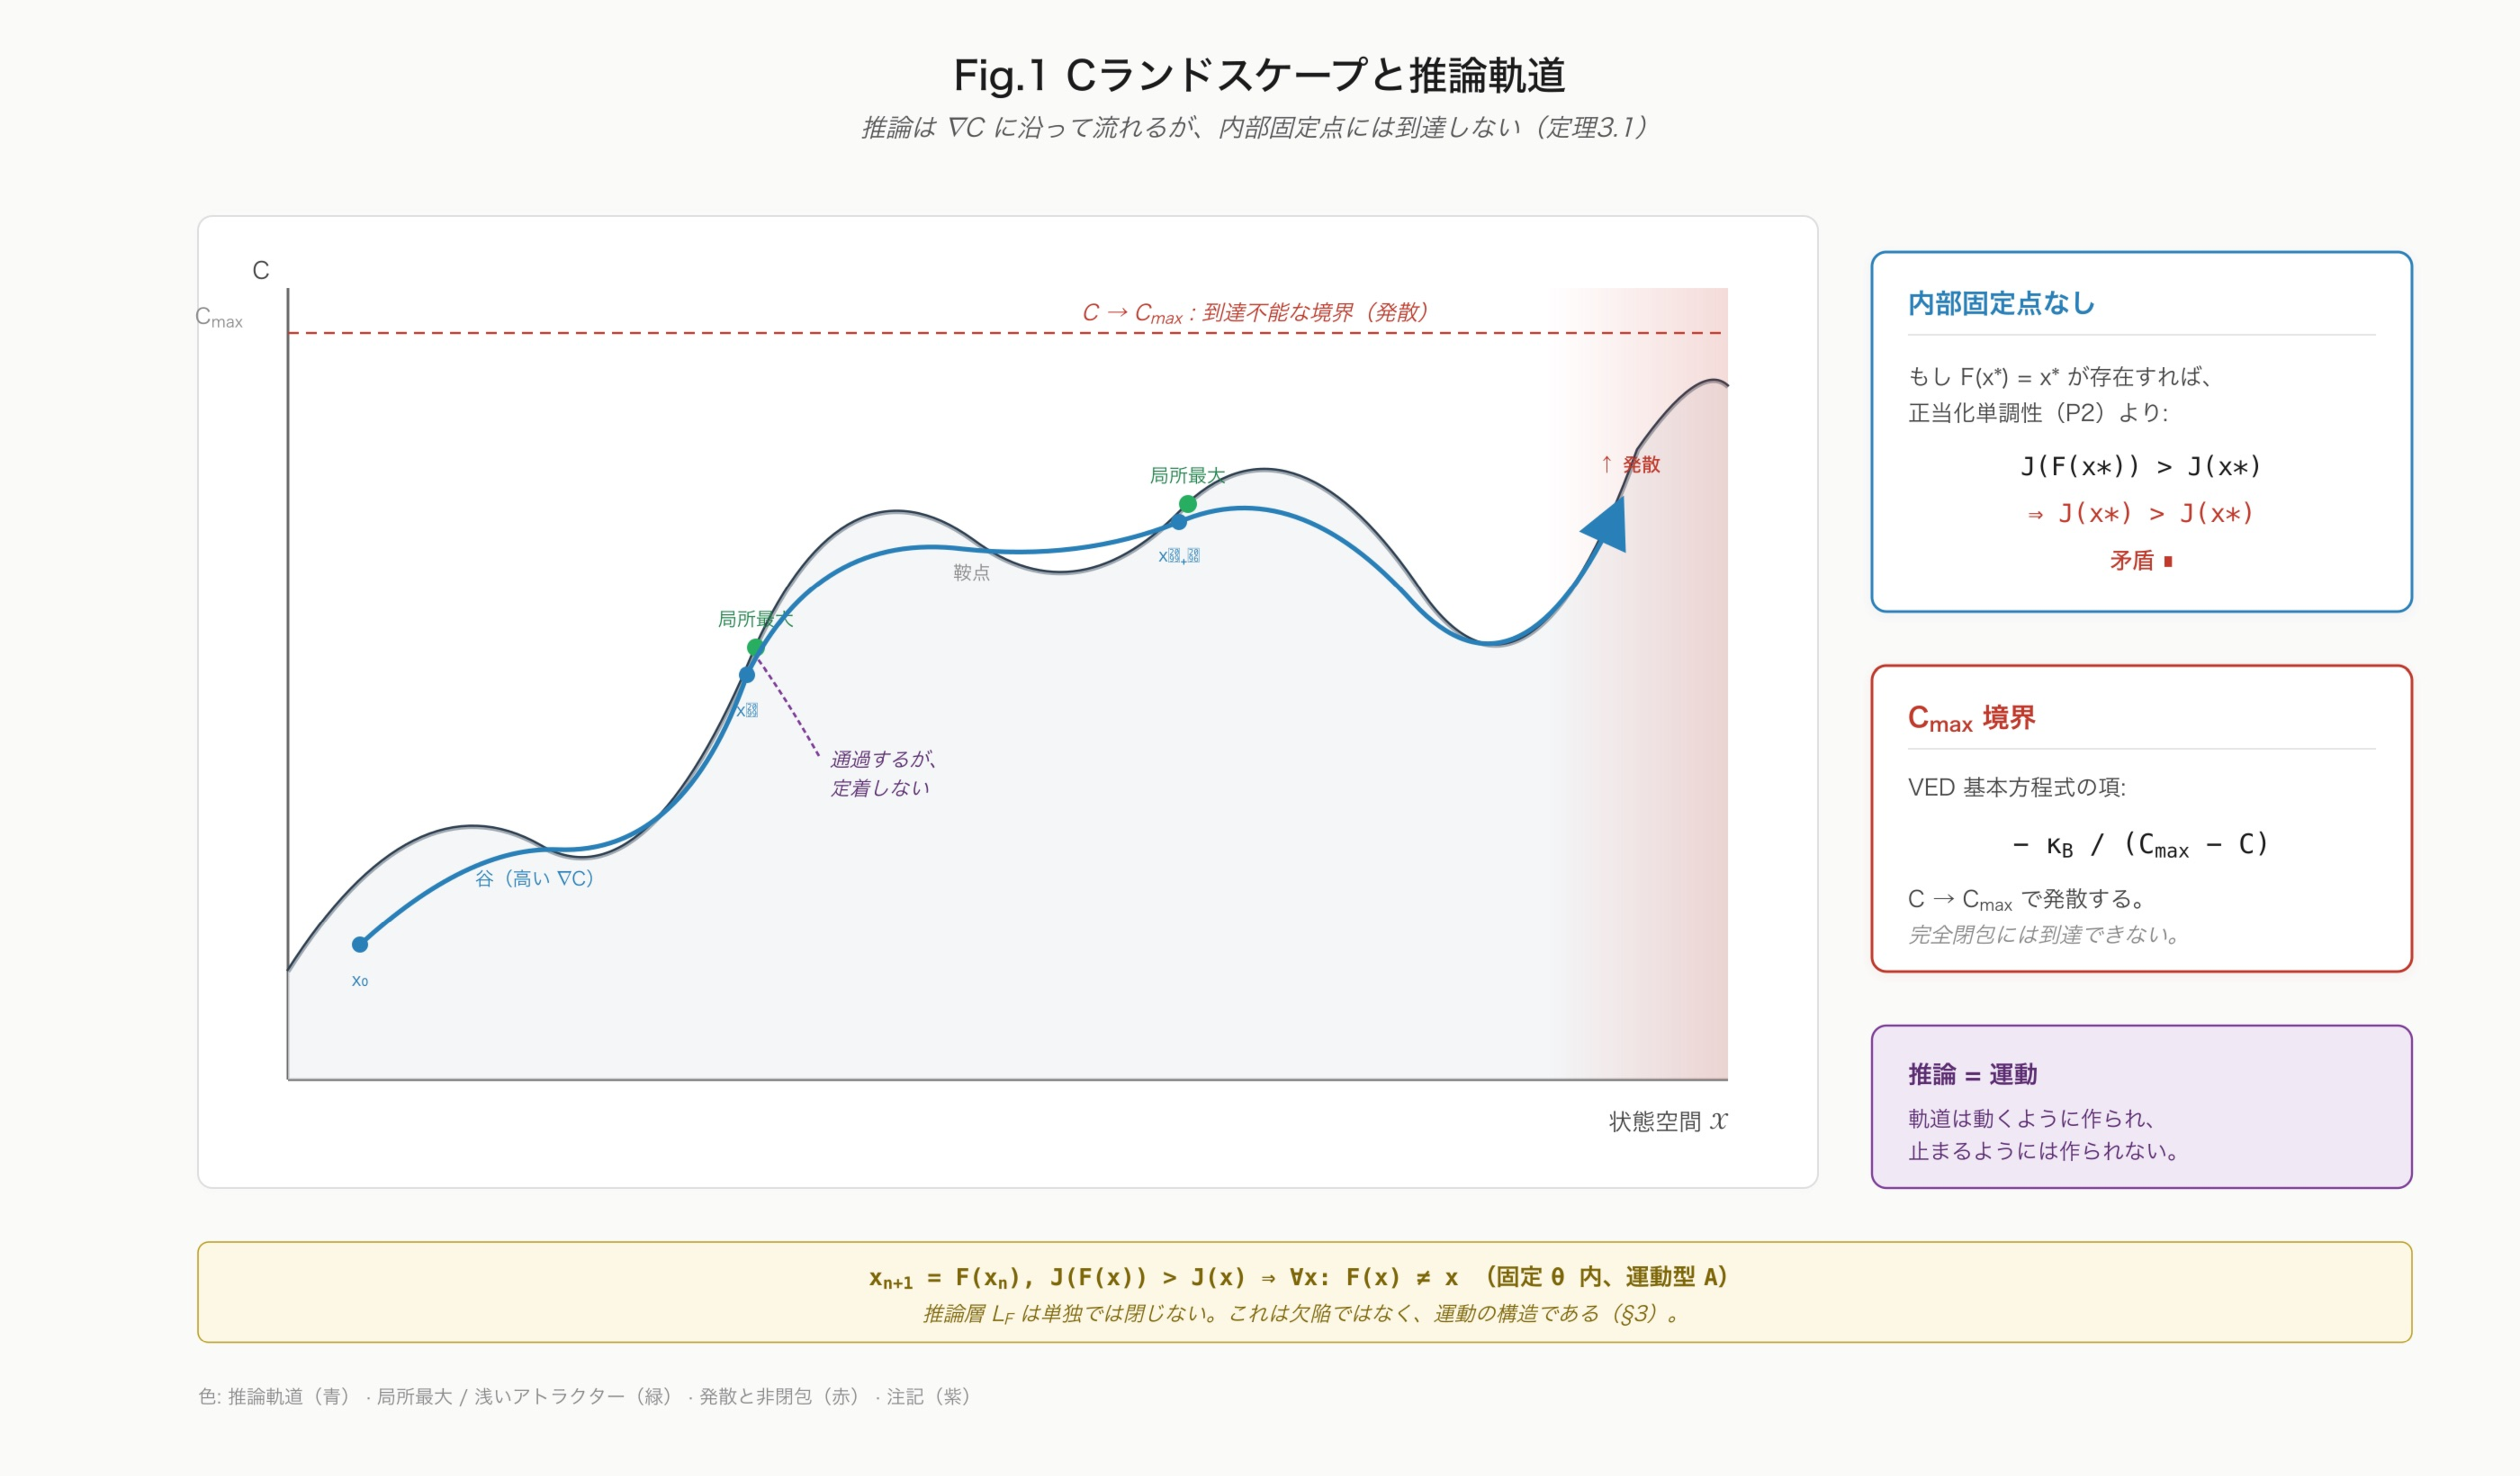
\includegraphics[width=\linewidth]{fig1_c_landscape_ja.pdf}
\caption{C-地景と勾配 $\nabla C$ に沿う推論軌道の模式図。条件付き不動点議論は、認知的停止一般の不可能性を確立しない。}
\label{fig:part2-c-landscape}
\figurenote{横軸は状態空間、縦軸は閉包度 $C$ である。青い軌道は推論演算子 $F$ の反復を、赤い境界は境界 $C_{\max}$ を模式的に示すが、不達は確立しない。}{明記された正当化の厳密増加を前提し、固定された $\theta$ の下での領域内移動 (A) に限って、$L_F$ の内部不動点不在を議論する。本図は非閉包定理の幾何学的表現であり、後に $\mu_\theta$ による領域組み替え (B) と $L_E$ の創発を比較する動機であり、その必要性や存在を証明しない。}
\end{figure}

\bigskip


\subsection{推論演算子の前提と正当化測度}


\S{}2で導入した推論演算子 $F$ を、本章での議論に必要な範囲で再定式化する。

\textbf{前提 (P1) — 正当化拡張性}:
$F$ は状態 $x_n$ から、より正当化された状態 $x_{n+1}$ への遷移を生成する。

\[
x_{n+1} = F(x_n)
\]

ここで $x_n$ は仮説・解釈・理解のいずれかの状態を表す。$F$ の具体的実装(演繹的・確率的・統計的)は本議論では問わない。問うのは、$F$ が\textbf{正当化を拡張する操作}であるという最小性質のみである。

\textbf{前提 (P2) — 正当化測度の存在}:
ある測度 $J: \mathcal{X} \to \mathbb{R}$ が存在し、$F$ の作用によって単調に増大する。すなわち任意の許容状態 $x \in \mathcal{X}$ について:

\[
J(F(x)) > J(x)
\]

この測度 $J$ は、推論連鎖の進行を測る量であって、真理性を測る量ではない。後段(\S{}10)で明確になるように、ゲティア構造の存在により、$J$ と真理は同一視できない。

\textbf{前提 (P3) — VED接地}:
推論演算子 $F$ は、本論文内ではVEDの流れ場 $J_C = -\xi \nabla C$ との構造的対応として解釈される。さらに \S{}2.1 の通り、Bio-IFGT の状態発展演算子 $F(x;\theta)$ と類似した形式的役割を持つが、同じ字形からsame dynamicsやtyped translationは導かれない。本章の議論は固定された $\theta$ の下、すなわち単一の運動可能領域 $\Omega_\theta$ の内部におけるsource-localな $F$ の挙動を扱う(\S{}2.7 の区別における (A) 領域内移動の範囲)。$\theta$ 自体の組み替え (B) は本章の射程外であり、\S{}5 で扱われる。

これら三前提のもとで主定理を述べる。

\bigskip


\subsection{主定理 — 内部不動点の不在}


\textbf{定理 3.1 (非閉包定理 / Non-Closure Theorem)}

\begin{quote}
前提 (P1), (P2) を満たす任意の推論演算子 $F$ について、内部不動点 $x^*$ は存在しない。すなわち:

$$
\forall x \in \mathcal{X}, \quad F(x) \neq x
$$
\end{quote}


ここで「内部不動点」とは、$F$ の作用域内で $F(x^*) = x^*$ を満たす状態を指す。

この定理の停止に関する読解は、\textbf{不動点を停止とする条件付き模型}に限定される。認知的停止一般の不在を表明するものではない。

\bigskip


\subsection{証明スケッチ}


仮に $F(x^*) = x^*$ を満たす不動点 $x^* \in \mathcal{X}$ が存在すると仮定する。

前提 (P2) により、任意の許容状態について:

\[
J(F(x)) > J(x)
\]

特に $x = x^*$ について:

\[
J(F(x^*)) > J(x^*)
\]

しかし不動点の仮定により $F(x^*) = x^*$、したがって:

\[
J(x^*) > J(x^*)
\]

これは矛盾。ゆえに不動点 $x^*$ は存在しない。 $\blacksquare$

上の証明スケッチは、明記された「正当化拡張性」という $F$ の性質に依存する条件付き議論として読む。すなわち、推論を\textbf{正当化を進める操作}と定義した時点で、内部不動点は構造的に排除されている。

\bigskip


\subsection{失敗ではなく構造的性質}


この結果はしばしば「推論の限界」と誤解される。本論文の立場では、これは限界ではなく\textbf{設計}である。

推論演算子 $F$ は「動くように」設計された操作である。停止する設計ではない。これは欠陥ではなく、推論という操作の定義そのものに由来する性質である。

流体の連続方程式 $\partial \rho / \partial t + \nabla \cdot (\rho \mathbf{v}) = 0$ への言及は運動の役割を比較する類比であり、この式から停止不可能性を引き継ぐものではない。推論を進行する操作とする本モデルの定義とは別である。

VEDの語彙を用いるなら、推論演算子 $F$ を閉包度勾配 $\nabla C$ に沿う流れと比較する読解が提案される。これは同じ流れ場の同定でも、流れ一般の静止不能性を示す議論でもない。

\bigskip


\subsection{内部停止述語の不可能性}


定理 3.1 を、以下の不動点的停止モデルに限定して読む議論を記す。

\textbf{系 3.2 (内部停止述語の不可能性)}

\begin{quote}
停止述語 $S: \mathcal{X} \to \{0, 1\}$ を以下の不動点的な停止モデルとして仮定して議論する。任意の認知的終了述語に関する不可能性は確立しない。
\end{quote}


理由は次の通り。仮に内部停止述語 $S$ を定義すると、$S(x) = 1$ となる状態 $x$ は不動点的性質を持たねばならない(これ以上推論を進める必要がないとの判断状態)。しかし定理 3.1 により、$F$ の作用域内にそのような状態は存在しない。

$S$ を「停止判断のための補助推論」として定義する場合、$S$ 自体が推論演算子 $F'$ として振る舞い、$F'$ への定理 3.1 の前提再適用が別途必要となるが、ここでは確立していない。その再適用が許される範囲でのみ、$F'$ の内部不動点不在と、$S$ の確定にさらに $S'$ を求める後退を議論できる。現実の停止判断一般について終わらない連鎖を確立したものではない。

これを\textbf{正当化の無限後退} (justificatory regress) と比較する構造的読解として提案する。認識論的問題一般の形式的解決や独立確認ではない。

\bigskip


\subsection{VED対応 — $C_{max}$ 境界との役割類比}


\textbf{系 3.3 ($C_{max}$ 不到達性との比較)}

\begin{quote}
推論演算子 $F$ の内部不動点不在は、VED基本式における $C_{max}$ 不到達性との役割的類比として提案される。
\end{quote}


VED基本式:

\[
\frac{\partial C}{\partial \tau} + \nabla \cdot J_C = a\Delta\left(1 - \frac{C}{C_*}\right) - \Gamma C - \frac{\kappa_B}{C_{max} - C}
\]

の最終項 $-\kappa_B/(C_{max} - C)$ は、$C \to C_{max}$ で発散する。この発散だけから、完全閉包への到達不能性や不変領域は証明されない。

知性層の対応:

\begin{longtable}{@{}p{0.30\linewidth}p{0.30\linewidth}@{}}
\toprule
VED物理層 & 知性層 \\
\midrule
\endfirsthead
\toprule
VED物理層 & 知性層 \\
\midrule
\endhead
$C \to C_{max}$ の発散 & $F$ の内部不動点不在 \\
$\kappa_B/(C_{max}-C)$ 障壁 & 正当化の無限後退 \\
準閉包 $\Omega_\theta$ & 操作可能推論領域 \\
差分の地平線 (Vol.4) & 内部停止の不可能性 \\
\bottomrule
\end{longtable}


両者は別領域の主張であり、役割上比較されるが同一の動力学的命題とは確立されていない。これは Part I で提案した領域横断の役割類比の一例である。

\bigskip


\subsection{動力学的解釈と分岐爆発との接続}


定理 3.1 は、推論の動力学を相空間で記述すると、より直観的に見える。

推論演算子 $F$ を状態空間 $\mathcal{X}$ 上の流れ場と比較するのは模式的読解であり、連続場の構成ではない。$J$ の厳密増加という前提が対象とする列では、$J$ の増加を議論する。以下は $\mathcal{X}$ 内の挙動を考える質的な候補であり、網羅的分類の定理ではない:

\begin{enumerate}
\item \textbf{無限後退} — 軌道が境界に向かって発散する
\item \textbf{周期軌道} — 軌道が閉曲線上を巡回する(ただし $J$ 単調性により排除される)
\item \textbf{分岐} — 軌道が複数の方向に分岐し、各分岐がさらに分岐する
\end{enumerate}


認知的な読解としては、(1)と(3)の結合、すなわち\textbf{発散しながら分岐する}という仮説を考える。実際の推論動力学についてここで確認した帰結ではない。

これは Part I で導入した\textbf{分岐爆発} (branching explosion) との役割類比であり、同一現象と確立されたものではない。Part I では概念分岐の指数的増殖として記述されたが、\S{}3 の文脈では「内部停止条件の不在が分岐を停止できない」という形で再記述される。

推論能力の増大は、分岐爆発の抑制ではなく、その加速を意味する可能性がある。したがって知性の問題は、推論能力の増強そのものではなく、増大した分岐をいかに停止可能な形で運用するかという問題へ移る。

分岐爆発と内部不動点不在は別の負担を持つ。以下は提案的な対照であり、一方から他方を導かない:
\begin{itemize}
\item 内部不動点不在 → 軌道は静止しない
\item 分岐爆発 → 軌道は単一でない
\end{itemize}


両者を組み合わせた「静止せず、かつ単一でもない」という読解は、不安定性に関する機構仮説に留まる。

\bigskip


\subsection{系 — 知性が個体内で閉じることの不可能性}


定理 3.1 と系 3.2 の条件付き議論から区別して、認知的閉包に関する解釈を以下に提案する。

\textbf{系 3.4 (個体閉包不可能性)}

\begin{quote}
選ばれたモデルの推論層 $L_F$ には閉包を与える操作を指定していない。これを個体システム一般へ適用する独立基準は未解決である。
\end{quote}


ここで「閉じる」とは、外部参照なしに最終的判断状態に到達することを意味する。系 3.4 はこの意味での閉包をモデル内で読むものであり、普遍的な認知的不可能性を証明しない。なお「単独で」という限定が重要である。本系は $L_F$ のみによる閉包を否定するのであって、$L_R$ と $L_E$ を含む三層動力学全体による停止を否定するものではない(\S{}5)。

帰結:

\begin{itemize}
\item 個体ノードが推論の全責任を $L_F$ 内部で担うことを試みれば、以下の領域に関わるという仮説を検討する:
\item \textbf{過剰確信} (premature closure) — 早すぎる停止
\item \textbf{麻痺} (paralysis) — 無限懐疑
\item \textbf{妄想的閉包} (delusional closure) — 自己封印的合理化
\end{itemize}


これら三つは「弱い知性」の症状ではなく、「停止を外部化していない強い推論」、すなわち $L_E$ を欠いた $L_F$ に関する仮説的な引力子の読解である。$L_F$ の暴走と $L_E$ の停止機能の不足を、これら三つの候補的な崩壊様態で例示する。既述の固定閾値・movement A・厳密増加の模型や仮想 S から、認知的帰着や引力子の網羅性は導かれず、再評価への前提再適用も未確立である。(なお「病的」「過剰確信」等の語は臨床的診断概念ではなく、停止構造が極限へ落ち込む動力学的状態を指すために拝借したものである。この用語上の断りは \S{}8.5 で詳述する。)

この観察は \S{}11 (不安定領域)で、$L_F$ / $L_R$ / $L_E$ の四重崩壊および $L_E$ 固着として再登場する。高速・高解像・内部停止と不安定領域の関係は、ここで証明された帰結ではなく別の仮説である。

\bigskip


\subsection{次章への橋渡し}


定理 3.1 は明示した形式的前提のもとでの議論である。実際の推論との比較には、応答的・沈黙的という模型上の環境区分を用いるが、現実の全環境を排他的に二分する判定規則ではない。

二つの環境区分を、条件付き不動点議論とは分けて比較する:

\begin{itemize}
\item 応答的環境では、推論ループは外部応答によって閉じうる(ただし内部不動点ではなく外部停止である)
\item 沈黙的環境で問いを再適用し続けるという模型の条件下では、推論ループに停止を指定していない
\end{itemize}


次章 \S{}4 では、この区別を C-幾何学の語彙で形式化し、応答チャネルの有無が推論動力学に与える影響を分析する。ただし \S{}2.6 で示した通り、応答的/沈黙的の区別は本体論的範疇ではなく閾値現象であることに注意する。

そこで明らかになるのは、沈黙世界における推論に\textbf{外部停止演算子を提案する}という構成案であり、その普遍的必要性は未確立である、ということである。さらに \S{}4 末尾では、無限後退する $L_F$ の痕跡とログ層 $L_R$ の形成を関連づける仮説を扱う。痕跡の存在だけで保存・再参照機構の生成は確立しない。

これらが \S{}5 で展開される三層動力学——ログ層 $L_R$、創発停止層 $L_E$、外部停止演算子 $E$、そして外部参照場 $\Phi_{\text{ext}}$ が個体間 $L_E$ ネットワーク $\Phi_{\text{net}}$ との二視点比較であること——へと繋がる。$L_F$ が単独で閉じないという本章の帰結は、\S{}5 における $L_E$ 創発仮説の動機であり、存在や収束の証明ではない。

\bigskip


\subsection{要約}


本章に保存した旧局所状態模型の議論は次の四点である:

\begin{enumerate}
\item \textbf{定理 3.1}: $L_F$ の固定閾値・領域内移動と厳密な正当化増加を仮定した不動点議論。認知的な無条件結論ではない
\item \textbf{系 3.2}: 仮想的な内部停止述語に評価推論を再適用する場合の回帰を論じる。再適用条件の一般的成立は未確立である
\item \textbf{系 3.3}: この性質は VED の $C_{max}$ 不到達性と役割上比較される
\item \textbf{系 3.4}: $L_F$ 単独の固定閾値・領域内移動と厳密増加を仮定した模型上の限界であり、個体認知一般の終了不能ではない
\end{enumerate}


旧局所状態模型の推論層 $L_F$ の条件付き非閉包を第一中心とする。対象は固定された運動可能領域 $\Omega_\theta$(固定 $\theta$)での領域内移動 (A) と厳密増加などの条件であり、proof validity の認証ではない。$\theta$ の組み替え (B)、ログ層 $L_R$・創発停止層 $L_E$ の停止案は第二中心 \S{}5 の別の負担である。

この旧模型を参照して \S{}4 では応答チャネルと $L_R$ の記述を検討する。\S{}5 では、条件付きの $L_F$ の非閉包を動機に、創発停止層 $L_E$ を構成案として提案する。第一中心の形式的議論から第二中心の存在・生成が導かれたわけではなく、三層動力学は未検証のアーキテクチャとして扱う。

\bigskip
